\documentclass[journal,12pt,twocolumn]{IEEEtran}

\usepackage{setspace}
\usepackage{gensymb}
\singlespacing
\usepackage[cmex10]{amsmath}

\usepackage{amsthm}

\usepackage{mathrsfs}
\usepackage{txfonts}
\usepackage{stfloats}
\usepackage{bm}
\usepackage{cite}
\usepackage{cases}
\usepackage{subfig}

\usepackage{longtable}
\usepackage{multirow}

\usepackage{enumitem}
\usepackage{mathtools}
\usepackage{steinmetz}
\usepackage{tikz}
\usepackage{circuitikz}
\usepackage{verbatim}
\usepackage{tfrupee}
\usepackage[breaklinks=true]{hyperref}
\usepackage{graphicx}
\usepackage{tkz-euclide}

\usetikzlibrary{calc,math}
\usepackage{listings}
    \usepackage{color}                                            %%
    \usepackage{array}                                            %%
    \usepackage{longtable}                                        %%
    \usepackage{calc}                                             %%
    \usepackage{multirow}                                         %%
    \usepackage{hhline}                                           %%
    \usepackage{ifthen}                                           %%
    \usepackage{lscape}     
\usepackage{multicol}
\usepackage{chngcntr}

\DeclareMathOperator*{\Res}{Res}

\renewcommand\thesection{\arabic{section}}
\renewcommand\thesubsection{\thesection.\arabic{subsection}}
\renewcommand\thesubsubsection{\thesubsection.\arabic{subsubsection}}
\newcommand*{\Perm}[2]{{}^{#1}\!P_{#2}}%
\newcommand*{\Comb}[2]{{}^{#1}C_{#2}}%
\renewcommand\thesectiondis{\arabic{section}}
\renewcommand\thesubsectiondis{\thesectiondis.\arabic{subsection}}
\renewcommand\thesubsubsectiondis{\thesubsectiondis.\arabic{subsubsection}}
\renewcommand{\complement}[1]{\widetilde{#1}}   

\hyphenation{op-tical net-works semi-conduc-tor}
\def\inputGnumericTable{}                                 %%

\lstset{
%language=C,
frame=single, 
breaklines=true,
columns=fullflexible
}

\begin{document}
\newtheorem{theorem}{Theorem}[section]
\newtheorem{problem}{Problem}
\newtheorem{proposition}{Proposition}[section]
\newtheorem{lemma}{Lemma}[section]
\newtheorem{corollary}[theorem]{Corollary}
\newtheorem{example}{Example}[section]
\newtheorem{definition}[problem]{Definition}

\newcommand{\BEQA}{\begin{eqnarray}}
\newcommand{\EEQA}{\end{eqnarray}}
\newcommand{\define}{\stackrel{\triangle}{=}}
\bibliographystyle{IEEEtran}
\raggedbottom
\setlength{\parindent}{0pt}
\providecommand{\mbf}{\mathbf}
\providecommand{\pr}[1]{\ensuremath{\pr\left(#1\right)}}
\providecommand{\qfunc}[1]{\ensuremath{Q\left(#1\right)}}
\providecommand{\sbrak}[1]{\ensuremath{{}\left[#1\right]}}
\providecommand{\lsbrak}[1]{\ensuremath{{}\left[#1\right.}}
\providecommand{\rsbrak}[1]{\ensuremath{{}\left.#1\right]}}
\providecommand{\brak}[1]{\ensuremath{\left(#1\right)}}
\providecommand{\lbrak}[1]{\ensuremath{\left(#1\right.}}
\providecommand{\cbrak}[1]{\ensuremath{\left\{#1\right\}}}
\providecommand{\lcbrak}[1]{\ensuremath{\left\{#1\right.}}
\providecommand{\rcbrak}[1]{\ensuremath{\left.#1\right\}}}
\theoremstyle{remark}
\newtheorem{rem}{Remark}
\newcommand{\sgn}{\mathop{\mathrm{sgn}}}
% \providecommand{\abs}[1]{\left\vert#1\right\vert}
% \providecommand{\res}[1]{\Res\displaylimits_{#1}} 
% \providecommand{\norm}[1]{\left\lVert#1\right\rVert}

% \providecommand{\mtx}[1]{\mathbf{#1}}
% \providecommand{\mean}[1]{E\left[ #1 \right]}
% \providecommand{\fourier}{\overset{\mathcal{F}}{ \rightleftharpoons}}

\providecommand{\system}{\overset{\mathcal{H}}{ \longleftrightarrow}}

\newcommand{\solution}{\noindent \textbf{Solution: }}
\newcommand{\cosec}{\,\text{cosec}\,}
\providecommand{\dec}[2]{\ensuremath{\overset{#1}{\underset{#2}{\gtrless}}}}
\newcommand{\myvec}[1]{\ensuremath{\begin{pmatrix}#1\end{pmatrix}}}
\newcommand{\mydet}[1]{\ensuremath{\begin{vmatrix}#1\end{vmatrix}}}
\numberwithin{equation}{subsection}
\makeatletter
\@addtoreset{figure}{problem}
\makeatother
\let\StandardTheFigure\thefigure
\let\vec\mathbf
\renewcommand{\thefigure}{\theproblem}
\def\putbox#1#2#3{\makebox[0in][l]{\makebox[#1][l]{}\raisebox{\baselineskip}[0in][0in]{\raisebox{#2}[0in][0in]{#3}}}}
     \def\rightbox#1{\makebox[0in][r]{#1}}
     \def\centbox#1{\makebox[0in]{#1}}
     \def\topbox#1{\raisebox{-\baselineskip}[0in][0in]{#1}}
     \def\midbox#1{\raisebox{-0.5\baselineskip}[0in][0in]{#1}}
\vspace{3cm}
\title{AI1103: Assignment 7}
\author{Chitneedi Geetha Sowmya \\ CS20BTECH11011}
\maketitle
\newpage
\bigskip
\renewcommand{\thefigure}{\theenumi}
\renewcommand{\thetable}{\theenumi}


Download all latex codes from 
\begin{lstlisting}
https://github.com/Geetha495/Assignment7/blob/main/Assignment7.tex
\end{lstlisting}
Download all python codes from 
\begin{lstlisting}
https://github.com/Geetha495/Assignment7/blob/main/Assignment7.py
\end{lstlisting}

\section{Problem}
Suppose $X$ is a positive random variable with the following probability density function,
\begin{align*}
f(x) = (\alpha x^{\alpha -1} + \beta x^{\beta-1} ) e^{-x^{\alpha}-x^{\beta}} ; x>0
\end{align*}
for $ \alpha >0, \beta >0$.
Then the hazard function of $X$ for some choices of $\alpha$ and $\beta$ can be
\begin{enumerate}
    \item an increasing function.
    \item a decreasing function.
    \item a constant function.
    \item a non monotonic function
\end{enumerate}
\section{Solution}
CDF of $X$, 
\begin{align}
    F(x) &=  \int_{-\infty}^xf(t)dt \\
    &= \int_{0}^xf(t)dt \hspace{1cm} \text{as } x>0\\
    &= \int_{-\infty}^t\left((\alpha t^{\alpha -1} + \beta t^{\beta-1} ) \times e^{-t^{\alpha}-t^{\beta}}\right)dt \\
    &= -e^{-t^{\alpha}-t^{\beta}} \Big|_0^x\\
    &= 1-e^{-x^{\alpha}-x^{\beta}}
\end{align}
Hazard function,
\begin{align}
    h(x) &= \frac{f(x)}{1-F(x)} \\
    &= \alpha x^{\alpha -1} + \beta x^{\beta-1} \\
    h^{\prime}(x) &= \alpha(\alpha -1) x^{\alpha -2} + \beta(\beta-1) x^{\beta-2}\\
     h^{\prime}(x) &= 
         \begin{cases}
    0 & \alpha=\beta=1 \\
    >0 & \text{otherwise}\\
    \end{cases}
    \end{align}
    Thus $h(x)$ can be either constant function or an increasing function.\\
    
    \begin{figure}[h]
    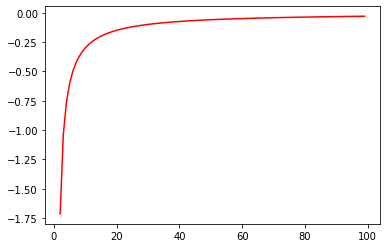
\includegraphics[width=8cm]{plot.png}
    \end{figure}
     From the above figure, it is verified that $h(x)$ can be either constant function or an increasing function.\\
       Correct options are 1,3.
\end{document}



